\documentclass{article}

% NeurIPS Creative AI track: standard NeurIPS style, ~4 pages excluding
% references. Swap neurips_2023 for the current year's official style file
% when available (the layout is unchanged year to year).
%   \usepackage{neurips_2023}            -> submission mode (anonymous, line numbers)
%   \usepackage[preprint]{neurips_2023}  -> preprint notice
%   \usepackage[final]{neurips_2023}     -> camera-ready
% NOTE: the repo only ships neurips_2023.sty; change to neurips_2026 on Overleaf.
\usepackage[preprint]{neurips_2026}
\usepackage[utf8]{inputenc}
\usepackage[T1]{fontenc}
\usepackage{hyperref}
\usepackage{url}
\usepackage{booktabs}
\usepackage{amsfonts}
\usepackage{amsmath}
\usepackage{nicefrac}
\usepackage{microtype}
\usepackage{xcolor}
\usepackage{graphicx}
\graphicspath{{figures/}}
\usepackage{algorithm}
\usepackage{algpseudocode}
\usepackage[normalem]{ulem}


% ---------------------------------------------------------------------------
% Draft scaffolding.
% \planned{...}  -> gray italic note for content still to be produced
% \resph{...}    -> gray placeholder for a pending NUMBER (fill when runs finish)
% \comment{...}  -> red margin-style note to co-authors
% \motif{...}    -> typeset an interval-class motif, e.g. \motif{0,3,-1,-1}
% ---------------------------------------------------------------------------
\newcommand{\planned}[1]{\textcolor{gray!70}{\textit{[Planned: #1]}}}
\newcommand{\resph}[1]{\textcolor{gray}{\texttt{[#1]}}}
\newcommand{\comment}[1]{\textcolor{red}{[#1]}}
\newcommand{\motif}[1]{\texttt{(#1)}}
\newcommand{\method}{MotiGen}

\newcommand{\cmtS}[1]{{\color{blue} (Simon: #1)}}


% Title: keep it interesting (people should want to read it).
% Alternatives considered -- pick one before submission:
%   "Hum a Few Bars: Motif-Conditioned Symbolic Music Generation with Attention Biasing"
%   "Composing with a Four-Note Seed: Steering Symbolic Music Models with Motifs"
% \title{\method{}: Motif-Conditioned Symbolic Music Generation with Attention Biasing}
\title{Getting Motif-ated: Controllable AI Compositions from Injected Motif Prompts}

% Creative AI track submissions are typically non-anonymous.
\author{%
  Chao Peter Yang \\
  Yale University\\
  New Haven, CT\\
  \texttt{chaopeter.yang@yale.edu} \\
  \And
    Cynthia Rudin \\
  Duke University\\
  Durham, NC\\
  \And
  Yue Jiang\\
  Duke University\\
  Durham, NC\\
  \AND
  Simon Mak\\
  Duke University \\
  Durham, NC
  \And
  Stephen Ni-Hahn \\
  Chinese University of Hong Kong, Shenzhen \\
  Shenzhen, Guangdong \\
}

\begin{document}

\maketitle

\begin{abstract}
Deep learning has transformed symbolic music generation by borrowing the training paradigms of large language models, with systems such as NotaGen now producing complete, stylistically convincing classical scores from a short prompt. These systems could become powerful creative partners, helping musicians generate endless possibilities. However, current systems expose almost no control handles on the music itself. In principle, control handles could be built into a foundation model trained from scratch, but this is rarely practical without massive amounts of quality annotated data and compute resources. We therefore present \method{}, a recipe for retrofitting pretrained symbolic music models to use new instruction prompts. \method{} injects a musical motif as a structured prompt line, reinforces it with a scalar attention bias toward the motif tokens, and learns the association with a two-phase curriculum. First it learns from focused excerpts cropped around motif occurrences in the training data, then full scores including the motifs. Our experiments show that our model composes with the prompted motif in over 92.3\% of generated pieces. Generated pieces using a variety of motifs are included in our sample site: https://motigen-site.github.io/.
\end{abstract}

%To exemplify our methodology, we instantiate it with the most natural unit of musical thought of the \emph{motif}, a short melodic pattern specified as a transposition-invariant sequence of notes or intervals.

%The realistic path to controllability is therefore to graft new control mechanisms onto an already-pretrained model.

%Control is limited to coarse metadata such as period, composer, and instrumentation, so a musician who has a melodic idea in mind has no way to make the model develop it, and naïvely pasting the idea into the prompt of a pretrained model forces the phrase to open the piece, greatly constraining how the idea can be used.

%State-of-the-art systems like NotaGen do not release their training corpora, and reproducing their scale of data and compute is out of reach for most researchers.

\section{Introduction}
\label{sec:intro}

Motifs are the atoms of musical composition. The four notes that open Beethoven's Fifth Symphony are among the most recognizable sounds in Western music, and nearly every bar of the movement grows out of them. Schoenberg called the motif the germ from which coherent musical form develops \citep{schoenberg1967fundamentals}. When composers have a musical idea, it usually arrives in exactly this form, where a handful of notes with a characteristic contour are developed into full-fledged pieces. Meanwhile, autoregressive language models trained on large score corpora \citep{huang2019music, payne2019musenet, wu2023tunesformer, qu2024mupt} now generate long, well-formed pieces. NotaGen in particular \mbox{\citep{wang2025notagen}} showed that the large language model (LLM) paradigm of pretraining, finetuning, and reinforcement learning carries over to musical scores in ABC notation, a textual representation of written music.%, with generated pieces rating competitively with human-composed classical music.

% \cmtS{we might want to be a bit more specific on limitations of existing approaches (avoid jargon, e.g., ``enharmonic spelling''). what are fundamental bottlenecks that prevent musicians from effectively using current AI tools for music composition? this then highlights the importance of our contributions.} 

However, few models give composers the option to control generation at the motif level, the granularity that would let composers develop vague musical ideas into full compositions. Existing control sits at two extremes, either having coarse controls such as style or genre, or needing fully formed musical ideas as input. Notagen \citep{wang2025notagen}, for example, limits the users to coarse inputs such as composer style, period, and instrumentation, offering no control over the development of musical material. Alternatively, the user might be expected to provide a concrete, full-fledged melody\citep{yuan2024chatmusicianunderstandinggeneratingmusic} to harmonize or a bar-level description sequence \citep{vonrutte2023figaro} that requires fully-composed material.

A motif, in its raw form, is an abstraction that is transposition invariant and may not even have defined intervals, so conditioning on a precise sequence of notes limits the generation. In trying to naively prompt existing models, we find that pretrained models ignore out-of-distribution prompt lines, so additional instructions must be taught without degrading the backbone's capabilities in generating music in general. Furthermore, judging whether a generated piece incorporates the motif well and consistently, requires specialized evaluation methods and careful examination.

We close this gap with \method{}. \method{} enables composers to build melodies and full pieces from a single abstract motif, represented as a transposition-invariant interval-class sequence of steps, skips, and leaps together with their contours. The motif is injected as a structured \texttt{\%motif:} prompt line in the score header. A scalar \emph{attention bias} at the motif line's key positions keeps the motif salient throughout decoding. A two-phase \emph{curriculum} teaches the model what the line means. Phase~1 fine-tunes on focused excerpts cropped from source pieces around located motif occurrences; phase~2 fine-tunes on full scores annotated with their extracted motifs. The result is a model that lets musicians develop ideas that are not yet fully formed, while retaining significant control over the piece's content. %four notes. %\footnote{While our motif identification algorithm supports various lengths, the authors has found that 4 note motifs tend to be the most abundant and easy to use}

%(e.g., \motif{0,3,-1,-1} would be a note, a leap up, then two steps down)

%, where the motif--content association is strong and local

Our novel contributions include: (1) a motif-conditioning method for symbolic music LLMs combining \texttt{\%motif:} prompt lines with a train- and inference-time attention bias, (2) a focused-crop curriculum that teaches motif grounding from phrases containing each motif and (3) a transposition-invariant, enharmonic-aware motif containment evaluator shared between training annotation and evaluation.

%, including a dose--response characterization of the bias strength

%(step/skip/leap classes, repeat collapse)

% adoption versus unconditioned base rates, ablations of bias and curriculum, the dependence of adoption on training-set motif frequency, and a Gradio co-composition interface. A real-data scaling study appears in Appendix~\ref{app:scaling}.

\begin{figure}[t]
  \centering
  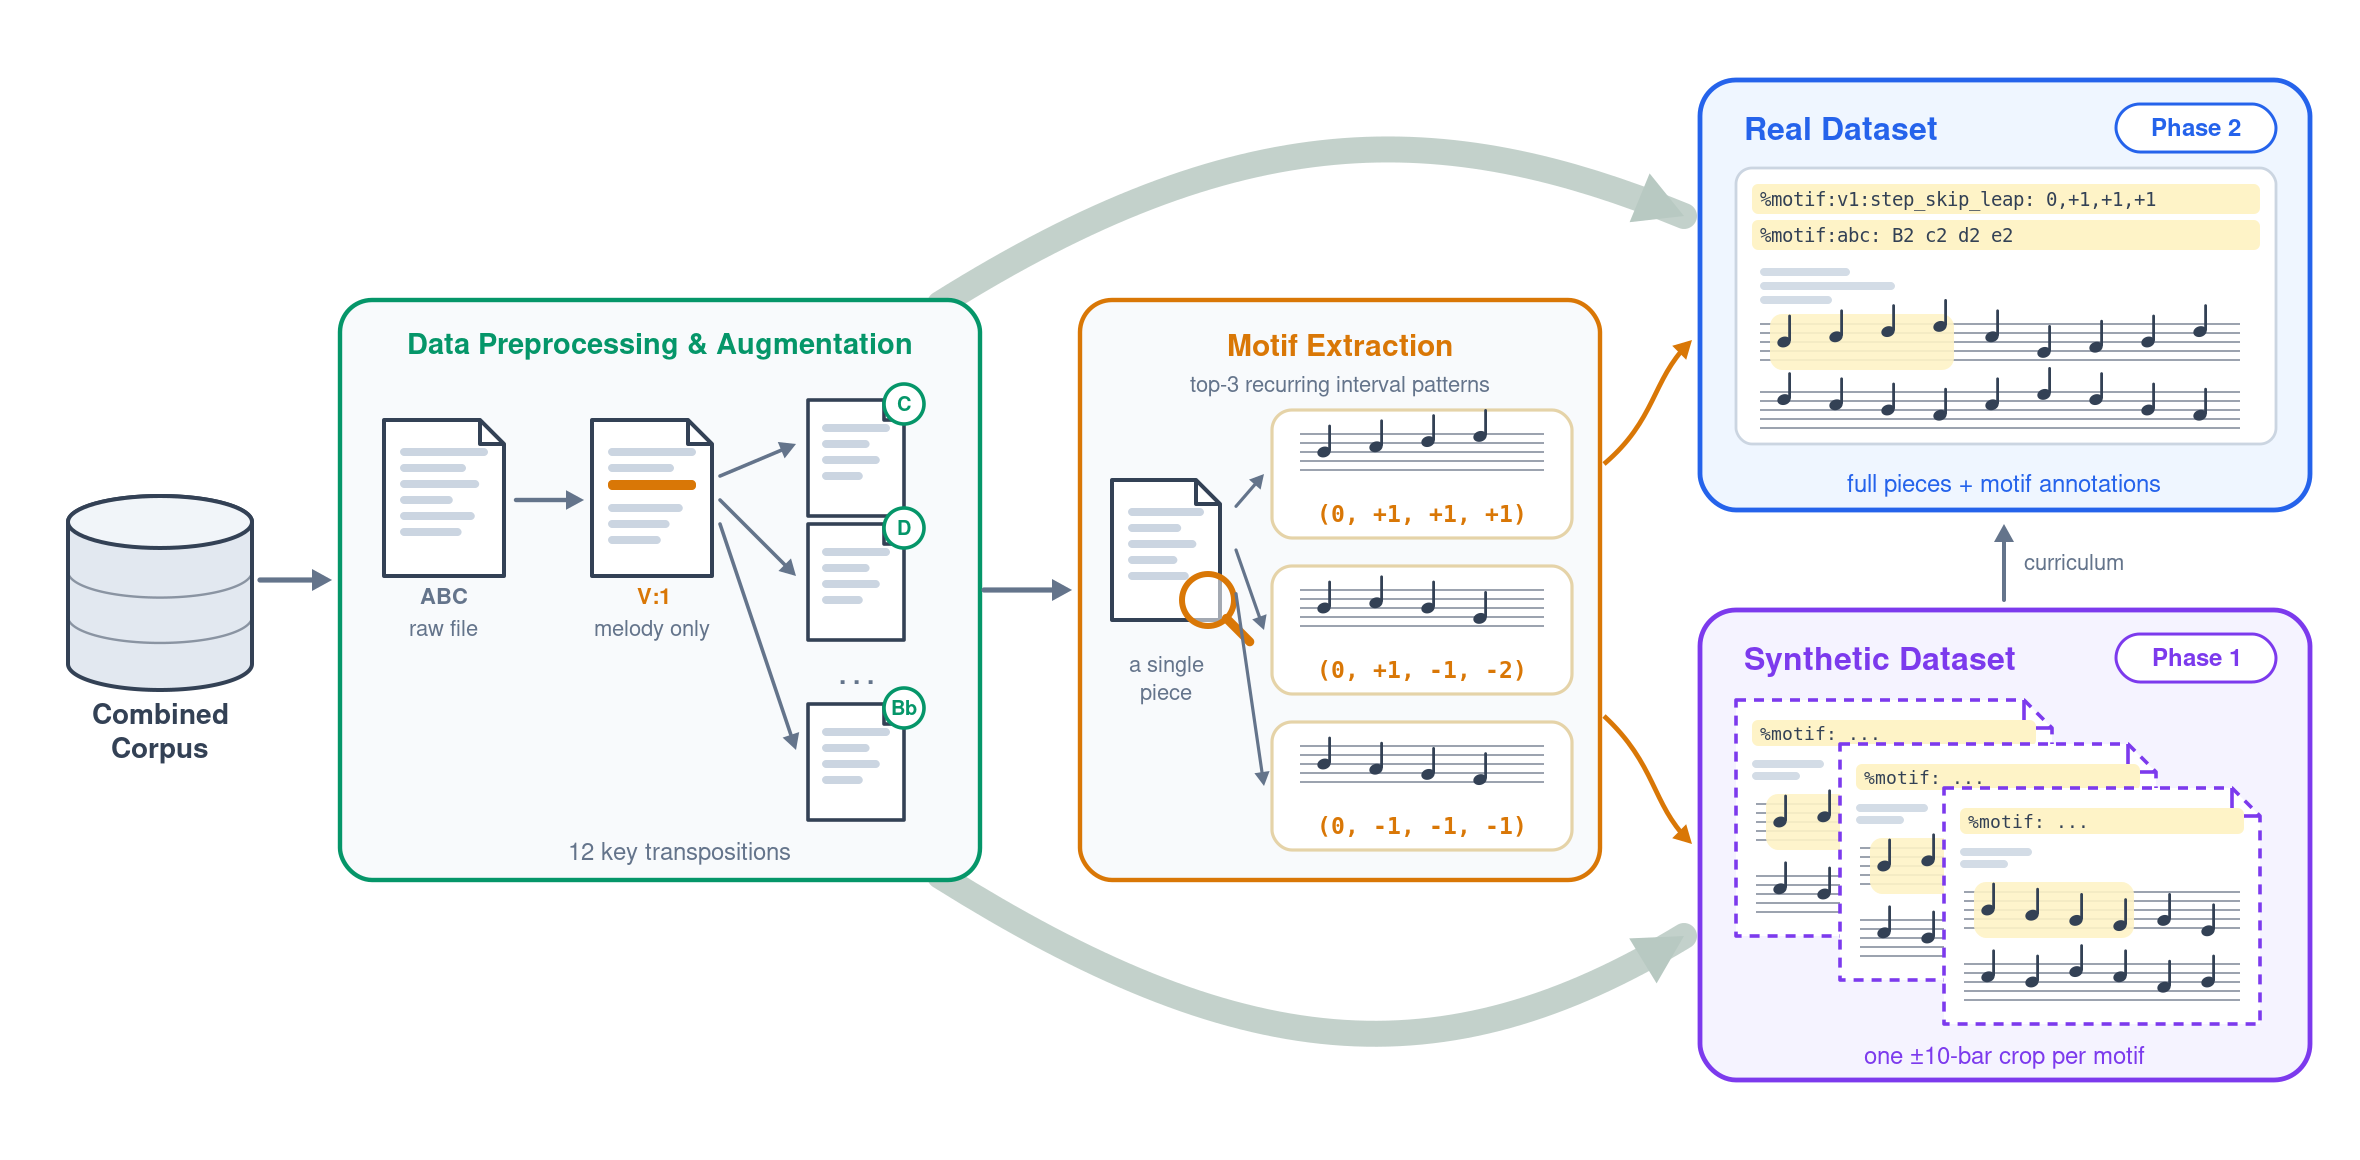
\includegraphics[width=\linewidth]{fig_1_pipeline.png}
  \caption{\method{} data pipeline: each piece is reduced to its melody line,
  augmented across keys, and mined for its recurring interval patterns; the
  located occurrences yield the phase-1 focused set of motif-centered crops
  and the phase-2 of full pieces with \texttt{\%motif:} annotations.} 
  \label{fig:overview}
\end{figure}

\section{Related Work}
\label{sec:related}

\subsection*{Generative Symbolic Music Models}
Autoregressive Transformers have long been applied to event-token and text-based score representations, from Music Transformer \citep{huang2019music} and MuseNet \citep{payne2019musenet} to ABC-notation models with bar/patch-aligned hierarchical decoding \citep{wu2023tunesformer, qu2024mupt}. NotaGen \citep{wang2025notagen} scales this lineage with LLM-style pretraining and preference optimization, and is the backbone for our experiments. None of these models provide control over thematic material.


%\subsection*{Controllable symbolic generation.}
Control has been investigated for deep learning music models via control tokens \citep{keskar2019ctrl}, learned description sequences \citep{vonrutte2023figaro}, text conditioning \citep{lu2023musecoco}, and hard structural constraints \citep{herremans2017morpheus}. While interpretable probabilistic frameworks give users direct, musically meaningful handles \citet{hahn2023interpretable,hahn2024senthymnent, nihahn2025progress}, they do not leverage the musical abilities of foundational music LLMs. The closest work to ours is Theme Transformer \citep{shih2022theme}, which conditions on a concrete theme involving specific pitches and rhythms and is trained from scratch. We instead condition on an \emph{abstract, transposition-invariant} pattern and retrofit the capability onto a pretrained LLM while preserving its fluency.


\subsection*{Attention and Activation Steering}
Classifier-free guidance \citep{ho2022classifier}, post-hoc attention steering (PASTA) \citep{zhang2024pasta}, and activation addition \citep{turner2023activation} modify a \emph{frozen} model's computation. Our bias is mechanically similar to PASTA's logit offset but is applied during training as well as inference, so the model learns to exploit the emphasized tokens. Our two-phase schedule is a curriculum \citep{bengio2009curriculum} in which short focused crops make the motif-content association explicit and direct before full-length scores dilute training with additional musical material.


\subsection*{Motif Discovery in Music Information Retrieval (MIR)} 

Repeated-pattern discovery is a classical MIR problem, from geometric methods such as SIA/SIATEC \citep{meredith2002algorithms} and their compression-oriented successors \citep{collins2013siarct} to interval-based melodic pattern analysis \citep{conklin2001patterns} and closed-pattern motivic analysis \citep{lartillot2005efficient}. The task has also been studied directly on audio \citep{nieto2014identifying} and remains an active benchmark problem with dedicated datasets \citep{hsiao2023bps} (see \citet{janssen2013discovering} for a survey). Our contribution is not the discovery algorithm, which, while novel in its representation of the motif, is a simple sliding-window extractor, but rather its use as an effective control signal for generation.

\section{Methodology}
\label{sec:method}

\subsection{Motif Representation and Extraction}
\label{sec:representation}

A motif must survive transposition and transformation. The opening four notes of Beethoven's Fifth is the same recognizable motif whether it starts on G or F, outlines a major or minor 3rd, or uses quarter notes instead of eighths. We therefore represent a motif not as pitches but as a sequence of \emph{signed interval classes} between consecutive melody notes, after collapsing immediate repetitions (see Figure~\ref{fig:encoding}). We measure the distance $d(\cdot,\cdot)\in\mathbb{Z}$ between two notes ($n_i$, $n_j$) in terms of diatonic scale steps. For example, $d(A\flat4,A\flat4)=0$, $d(A\flat3,B\flat3)=1$, and $d(C5,F4)=-4$. Intervals are then classified as \textit{steps} when $|d|=1$, \textit{skips} when $|d|=2$, and \textit{leaps} when $|d|\geq3$. We focus on pitch-based motifs and ignore note repetitions, so an interval class for $d=0$ is not required. Rather, we use 0 as a placeholder for the first note of a motif. For example, \motif{0,3,-1,-1} encodes a starting note, a leap up, and two steps down, respectively. The representation is transposition-invariant by construction and deliberately coarse. It captures contour and interval category, which is what most listeners track when they recognize a motif across keys and harmonizations.

%Each diatonic letter-step distance $d$ maps to $\operatorname{sign}(d)\cdot\{1,2,3\}$ for a step ($|d|{=}1$), skip ($|d|{=}2$), or leap ($|d|{\geq}3$), with a leading $0$ anchoring the first note.

To extract the motif from a piece, we use a sliding-window parser. We scan each piece end-to-end using a window length of 4--10 notes, and keep a count of each note sequence's occurrence throughout each piece. We select the most common sequence (weighted by length to mitigate inherent bias towards shorter motifs) to be a defining motif of the piece. We find motifs of four notes. Repeats and ornamentation are ignored throughout this process in order to avoid fragmenting motif counts. This extraction technique is used to annotate training data and evaluate generated results (details in Appendix~\ref{app:extraction}).

%Interestingly, even with the weighting, we still found that most pieces tend to produce motifs of length 4. Therefore, to reduce biases in data, avoid fragmentation, and limit burden on the model, the authors have deiced to use motifs of length 4 throughout the paper.

\begin{figure}[t]
  \centering
  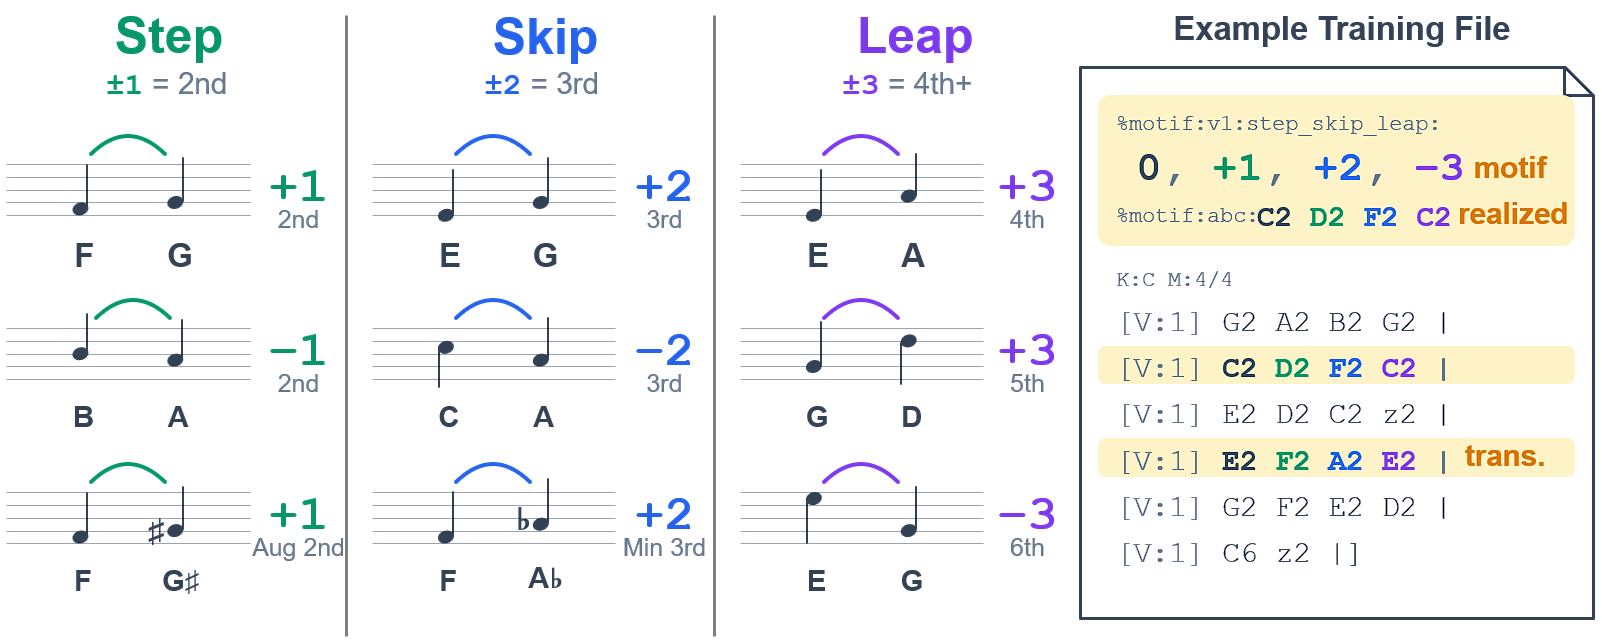
\includegraphics[width=0.95\linewidth]{fig_3_encoding.png}
  \caption{Interval-class encoding. Left: signed letter-step distances map to
  steps ($\pm1$), skips ($\pm2$), and leaps ($\pm3$). The classification is
  diatonic, so an augmented second is a step while its enharmonic minor third
  is a skip. Right: the resulting \texttt{\%motif:} prompt lines in a
  training file, with the realization and a transposed recurrence of the
  same pattern highlighted.}
  \label{fig:encoding}
\end{figure}

\subsection{Conditioning Interface}
\label{sec:conditioning}

\textbf{Novel Prompt Lines:} The motif is injected as structured comment lines prepended to the ABC header, replacing NotaGen's period--composer--instrumentation prompt. Concretely, we add \texttt{\%motif:v1:step\_skip\_leap: 0,3,-1,-1} as the abstract motif for voice \texttt{V:1}, and optionally \texttt{\%motif:abc: G B d c} as one concrete realization (see Figure~\ref{fig:encoding}, right). During inference, the model can be run \emph{abstract-only}, where the user provides the abstract motif, and the model will subsequent output the musical phrase containing the actual motif (the realization). Alternatively, the user could also provide the actual motif for \method{} to use.

\textbf{Motif Attention Bias:} A prompt line alone competes with hundreds of body tokens and its influence decays over a long generation. We therefore add a scalar bias $\beta$ to the pre-softmax attention logits at the motif prompt's key positions in the patch-level decoder $\alpha_{ij} = q_i^\top k_j/\sqrt{d} + \beta\cdot\mathbf{1}[j \in \mathcal{M}]$, where $\mathcal{M}$ is the set of patch positions belonging to \texttt{\%motif:} lines. The bias is applied identically at training and inference, so the model learns calibrated use of the emphasized channel rather than having its attention distorted post hoc (Figure~\ref{fig:training}, bottom). We find that the optimal bias strength for our case is $\beta{=}4$, while $\beta{=}2$ has little effect, and $\beta{\geq}8$ collapses generation entirely (more details in Section~\ref{sec:ablations}).

\subsection{Curriculum training}
\label{sec:curriculum}

To ease the model into learning new prompt material, we structure training with a two-phase curriculum (overview in Figure \ref{fig:training}, top).


\textbf{Phase 1 (Focused Crops):} For every located motif occurrence in the source corpus we build focused cropped training data. The surrounding phrase, cropped to $\pm$5 measures around the occurrence, includes the full original header plus the motif prompt lines. Because these excerpts are real music centered on the motif instead of algorithmically generated samples, the distribution of training data does not drift far from full human-composed pieces. This phase allows the model learn the association between the motif prompts and the generated content of the music more directly.

\textbf{Phase 2 (Full Pieces):} We then fine-tune on full-length scores, each annotated with its extracted motif, with the attention bias active. Here, the model learns how the motif should be present and varied throughout the piece. Curriculum training implementation is detailed in Appendix \ref{app:curriculum_implementation}.


\begin{figure}[t]
  \centering
  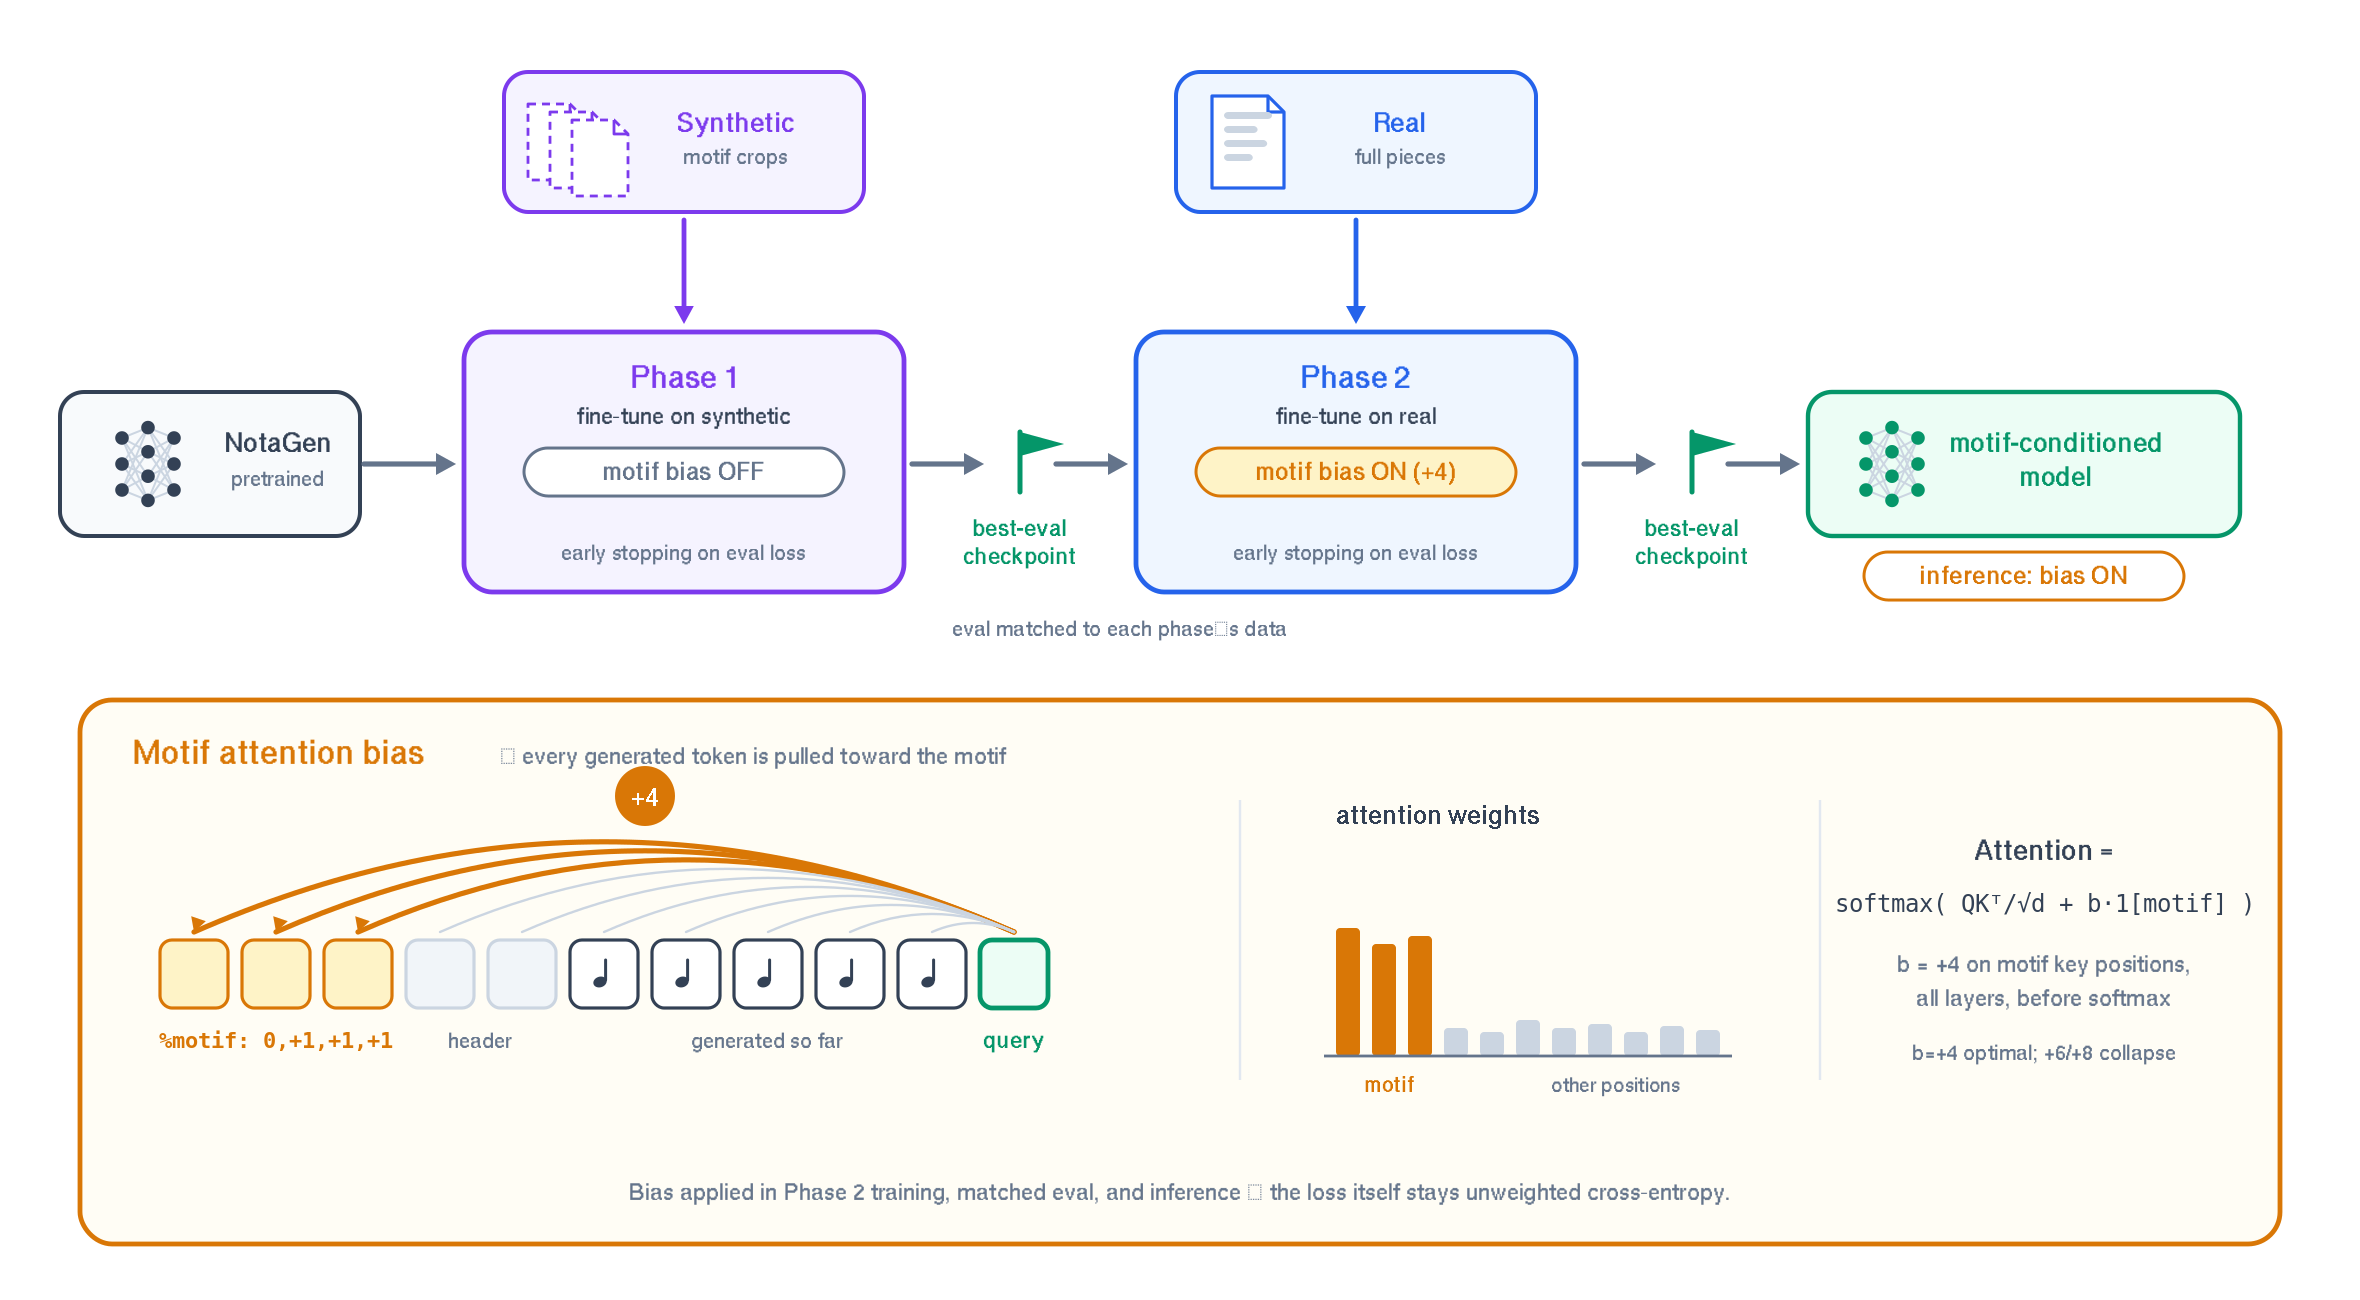
\includegraphics[width=0.95\linewidth]{fig_2_training.png}
  \caption{Two-phase curriculum with phase-matched evaluation (top) and an illustration of the
  motif attention bias (bottom), where a scalar $\beta$ added to the pre-softmax
  attention logits at the \texttt{\%motif:} key positions, identically at
  training and inference.}
  \label{fig:training}
\end{figure}

\subsection{Training Datasets and Motivic Analysis}
\label{sec:data}

We build on NotaGen \citep{wang2025notagen}, pretrained on $\sim$1.6M ABC-notation pieces and fine-tuned by its authors on $\sim$9k classical scores with period--composer--instrumentation prompts; all of our training modifies this checkpoint. Our source-data pool combines the OpenScore Lieder corpus \citep{gotham2022lieder} ($\sim$1.3k Romantic-era songs, from which we take the \texttt{V:1} vocal line) with the Irishman corpus \citep{irishman2023} of 216k+ monophonic folk tunes, each wrapped into a single-voice score so both sources share one format, these pieces are then augmented across 12 keys as shown in Figure~\ref{fig:overview}. The focused cropped phase-1 set consists of $\sim$650k+ motif-centered crops built from the same pool (Section~\ref{sec:curriculum}). Given the available dataset, the model will be trained to be monophonic only. In future works, when comparable or larger homophonic datasets becomes available, we plan to expand the model to generate multiple voices as well.
% TODO: pull final counts from build logs (corpus-composition table cut for now).
An exploratory analysis of the extracted motifs motivates our evaluation design: the source pool contains 210 distinct length-4 motif patterns whose frequencies are strongly skewed. Stepwise descent \motif{0,-1,-1,-1} occurs 62{,}356 times, the rank-27 pattern appears 1{,}083 times, and pure leap chains such as \motif{0,3,3,3} appearing twice in the entire pull (details in Appendix \ref{app:motif_analysis}). We therefore stratify our evaluation based motif frequency.
% Optional if space allows: small log-log rank--frequency figure (could go in
% the appendix instead).
%Any claim about motif conditioning therefore has to be stratified by training frequency, which our evaluation does explicitly.

\section{Experiments}
\label{sec:experiments}

%designed a series of evaluations and experiments to quantify the motif-related musical performance of the model. 

To evaluate \method{}, our experiments investigates how well \method{} can reliably compose music that organically integrates a prompted motif. We break this down into the following manageable questions: (1)~To what extent do our methods increase the model's performance? (Section~\ref{sec:ablations}), (2) how does performance scale with full-data quantity (Appendix~\ref{app:scaling}), and (3) Does \method{} incorporate the motif musically into the generated piece? We provide a case study of results in Section \ref{sec:case}, and plan for larger scale human evaluation in future works. 

% \subsection{Experimental setup}
% \label{sec:setup}

For each (model, motif) pair we generate 50 pieces with the abstract-only prompt and fixed decoding (top-$k{=}9$, top-$p{=}0.9$, temperature $1.2$), matching NotaGen's recommended sampling settings. The resulting samples are then evaluated using two metrics, one is \textit{body containment}, which asks whether the generated melody contains the target pattern anywhere, according to the motif extractor of Section~\ref{sec:representation}. Another is \textit{realization faithfulness}, which asks whether the model's own emitted \texttt{\%motif:abc} line realizes the target. Their $2\times2$ crosstab separates a model that understands a motif from one that further composes with it. The motifs used in experiments span the training distribution, namely we draw a stratified sample consisting of eight from the top-10 (band A) most frequent patterns, eight mid-distribution patterns (ranks 11--40 of 210, band B), and eight from ranks 41 and rarer (band C).


\subsection{Ablations}
\label{sec:ablations}

We ablate attention bias and curriculum training on the same protocol (Table~\ref{tab:ablation}). To test the efficacy of attention bias, we perform curriculum training with bias $\beta{=}0$ during both training and inference. To examine the benefits of curriculum training, we remove the cropped-data training phase, fine-tuning only on full pieces. Lastly, we judge performance after ablated both attention bias and cropped-data training phase. 

Results provide strong evidence that our full recipe is effective based on all three metrics. Furthermore, each ablated component is shown to positively contribute to motivic composition. Removing the attention bias costs the most while removing the cropped training phase has a milder effect on mid-distribution motifs. The cropped phase matters far more for motifs from the distribution tail and at small corpus scale (Appendix~\ref{app:scaling}). Interestingly, plain fine-tuning on the annotated corpus already reaches 79.4\% containment against a 35.9\% base rate. So it seems the prompt format itself is learnable from data alone, and the motif bias and curriculum training are complementary rather than additive; the cropped curriculum with the bias removed performs no better than plain fine-tuning, whereas together they lead on every metric. 


% Latest experimental results
\begin{table}[t]
  \centering

  \small
  \begin{tabular}{lccc}
    \toprule
    Configuration & Containment & Faithfulness & Motifs / Measure \\
    \midrule
    \method{} (bias $\beta{=}4$ + curriculum) & \textbf{92.3\%} {\scriptsize[90.7, 93.7]} & \textbf{93.0\%} {\scriptsize[91.4, 94.3]} & \textbf{0.25} \\
    \quad $-$ attention bias                  & 77.8\% {\scriptsize[75.4, 80.1]} & 75.8\% {\scriptsize[73.3, 78.2]} & 0.18 \\
    \quad $-$ cropped phase                 & 86.7\% {\scriptsize[84.6, 88.5]} & 87.2\% {\scriptsize[85.2, 89.0]} & 0.22 \\
    \quad $-$ both                            & 79.4\% {\scriptsize[77.0, 81.6]} & 76.1\% {\scriptsize[73.6, 78.4]} & 0.19 \\
    Base rate (no motif prompt)               & 36.8\% {\scriptsize[34.1, 39.5]} & --- & 0.06 \\


    \bottomrule
  \end{tabular}
\caption{Ablation of \method{} components: body containment (the piece
  contains the motif at least once) and realization faithfulness, averaged over the 24 stratified sample motifs at $n{=}50$ per motif. $\beta{=}4$ configurations use training-matched bias application at inference. Bracketed values are $95\%$ Wilson score intervals on the pooled counts ($n{=}1200$). See Appendix ~\ref{sec:eval} for the definitions of Containment and Faithfulness. 
  \label{tab:ablation}}
\end{table}

\subsection{Case Study}
\label{sec:case}
\begin{figure}
    \centering
    \includegraphics[width=0.95\linewidth]{fig_4_comparison.png}
    \caption{Excerpts from \method{} (upper) and Fable 5 (lower) when prompted to generate a melody with the motif of a leap up, and two steps down.}
    \label{fig:comparison}
\end{figure}

In order to get a better understanding of the subjective, qualitative qualities of the music generated by \method{}, both by itself, and in context of other methods, we provide a case study to examine a piece generated by \method{}. We prompt the model with a somewhat common, mid-distribution motif of (0, 3, -1, -1), which is a leap up, and two steps down, and allow the model to generate the realization, key signature, and time signature freely. 

Since no model to our knowledge generates music based on the same level of abstraction, we prompt a state-of-the-art general-purpose LLM, Fable 5 \citep{anthropic2026fable5}, with the following prompt and default settings to produce a comparable piece of music: 
\begin{verbatim}
        Generate a melody with a motif that goes a leap up
        and two steps down. Feel free to use any key signature
        or time signature, output in ABC notation.
\end{verbatim}
Figure \ref{fig:comparison} shows the melody generated by \method{} not only includes the motif as expected, but also includes interesting and diverse rhythms, as opposed to the simple quarter note sequence as created by the Fable 5 model. The realization of the motif is also more diverse in the sample generated by \method{}, as it includes both a leap with 6th (measure 1 -2), and a 5th (measure 2), while all the motifs in the sample by Fable 5 are all a 6th up and two steps down. Not to mention, the Fable 5 composition contains only the motif and nothing else other than the small cadence in measure 4, while \method{} has ample connecting materials between occurrences of the motifs.


% \begin{figure}[t]
%   \centering
%   % Spec: listening-study results -- musicality preference, motif salience
%   % (conditioned vs. unconditioned), and integration ratings, with CIs;
%   % fonts >= body size.
%   \fbox{\parbox{0.9\linewidth}{\centering\vspace{0.8em}
%   \planned{human listening study: musicality preference, motif salience,
%   integration ratings}
%   \vspace{0.8em}}}
%   \caption{Human listening study results. \resph{placeholder}}
%   \label{fig:human}
% \end{figure}

% \section{Creative Application}
% \label{sec:demo}

% \method{} is built to sit inside a composer's loop, and samples from these generations can be found on our sample site. The user supplies a motif, an abstract contour like \motif{0,3,-1,-1} or a concrete ABC snippet, then picks a period, composer, and instrumentation, and receives an engraved score with synthesized audio. Because the motif is the stable element across re-rolls, iteration is meaningful: re-generate with the same motif until a setting resonates, then tweak the motif to explore neighboring ideas. Thematic authorship stays with the human, while the model drafts continuations, figuration, and formal scaffolding. The abstract-contour entry point matters most for non-experts, since omeone who cannot notate music can seed a full piece from a shape they can hum.

% \section{Limitations}
% \label{sec:limitations}

% \cmtS{don't think we need this as an explicit section - can summarize \& integrate into earlier sections} Our conditioning and evaluation are single-voice. Multi-voice motif placement is untested at scale. Containment is necessary but not sufficient for musical use of a motif; we do not yet measure development or variation, where much of the compositional art lies. Rare-motif conditioning remains near floor, limiting out-of-distribution creative control. Finally, our automatic evaluation is a lexical containment check at a single decoding configuration. 


%All training data is public-domain or openly licensed (OpenScore Lieder, Irishman); the backbone follows NotaGen's data statement. Style-conditioned generation raises legitimate concerns about imitation and creative labor; \method{} is positioned deliberately on the composer-in-the-loop side of that line. The majority of the load-bearing creative decision and thematic material, comes from the human. The primary beneficiaries we envision are musically inclined people without formal training, for whom hearing their own idea developed has historically required years of technique.

\section{Conclusion}
\label{sec:conclusion}

We introduce \method{}, a recipe for retrofitting a thematic-control channel onto a pretrained symbolic music model by representing the motif as a transposition-invariant interval-class pattern, injecting it as a structured prompt line, reinforcing it with a matched train/inference attention bias, and training it with a focused-crop curriculum. Our resulting model composes convincing music with motivic material organically integrated into the texture rather than simply appended to the beginning. The same recipe could carry other musical instructions: harmonic progressions, bass lines, rhythmic cells, formal plans. %Every tool that has broadened who gets to make music started by shrinking the distance between an idea and the final product.


\bibliographystyle{plainnat}
\bibliography{references}

\appendix

\section{Implementation Details}
\label{app:curriculum_implementation}

For curriculum learning, checkpoints are selected by early stopping on held-out loss, and evaluation is phase-matched. Each phase is evaluated on data from its own distribution and in its own bias configuration. Evaluating a bias-trained model with the bias off understates its quality and distorts the training curve; matching removes a spurious cross-phase jump that would otherwise suggest phase~2 begins by ``undoing'' phase~1. Figure~\ref{fig:training} summarizes the schedule.

\paragraph{Training configuration.}
All fine-tuning starts from the public NotaGen-large checkpoint (20-layer patch-level encoder, 6-layer character-level decoder, hidden size 1280, patch length 1024, patch size 16) in NotaGen's patch-streaming regime, using AdamW with learning rate $10^{-5}$ and batch size 1. Each curriculum phase runs for up to 10 epochs with early stopping on held-out loss. Every training run fits on a single NVIDIA RTX A6000 (48\,GB) within a 48-hour budget; the reported experiments (the ablation grid of Table~\ref{tab:ablation}, the scaling grid of Appendix~\ref{app:scaling}, and their 50-piece-per-motif evaluation sweeps) total roughly one GPU-month on this hardware, and exploratory runs not reported in the paper required a comparable additional amount.

\paragraph{Code and sample release.}
The motif extraction and containment evaluator used both to annotate the training data and to compute every reported metric is publicly available at \url{https://github.com/cpyang123/motigen}, together with annotated training-data samples, the twenty generated pieces showcased on the demo site, and a notebook that extracts motifs, counts occurrences, and engraves scores with each motif occurrence highlighted. Generated pieces with in-browser playback are at \url{https://motigen-site.github.io/}. The fine-tuned model weights and the training pipeline are not part of this release.

\paragraph{Broader impact.}
All training data is public-domain or openly licensed (OpenScore Lieder, Irishman); the backbone follows NotaGen's data statement. Generative music raises legitimate concerns about imitation and creative labor; \method{} is positioned deliberately on the composer-in-the-loop side of that line, as the load-bearing creative decision, the thematic material, comes from the human. The primary beneficiaries we envision are musically inclined people without formal training, for whom hearing their own idea developed has historically required years of technique.

\section{Data scaling improves motif adoption}
\label{app:scaling}

Beyond the main ablations, we ask whether motif adoption improves with more training data, holding the recipe fixed. To do this, we train all the model variants, ablated models and the full model, on two subsets of the training data. Specifically, a 10k subset that is an order of magnitude smaller than the 200k+ full dataset, and a 1k dataset that is another order of magnitude smaller still. Additionally, in order evaluate the models performance on motifs of different obscurity, we do the same stratified sample of 8 motifs from the top 10 motifs in the full dataset, middle 11-40 motifs, and the tail 41+ motifs, corresponding to A, B, and C respectively as in Table \ref{tab:scaling}. Each motif is sampled 50 times, and the score calculated as an average over all the generated pieces. The Full Training block reports the underlying component results of Table \ref{tab:ablation}.


\subsection{Full per-motif results}
\label{app:tables}

Closely examining Table \ref{tab:scaling} reveals quickly that the full advantage of the full training pipeline is greatest when we have few data points, second when we have relatively abundant data, and worse when the paucity of data greatly hinders generalization across all configurations. 

Utilizing the entirety of the training regiment almost unanimously provides better results when trained over the 10k subset and the full training dataset. This is especially prominent when looking at the generations using motifs from the tail-end of the distribution, those of rank C. When prompted with these motifs, the full training recipe produces almost consistently a 10\% improvement in both containment and faithfulness over the next best ablation configuration when trained on either the full and the 10k dataset. This could indicate a better internal understanding of the motivic structure and its relation to the generated piece, leading to better generalization on sparser data. 


\begin{table}[h]
  \centering
  \small
  \begin{tabular}{lcccccc}
    \toprule
    & \multicolumn{3}{c}{Containment (\%)} & \multicolumn{3}{c}{Faithfulness (\%)} \\
    \cmidrule(lr){2-4}\cmidrule(lr){5-7}
    Configuration & A & B & C & A & B & C \\

    \midrule
    \multicolumn{7}{l}{\emph{$1$k source training pieces}} \\
    \method{} (full recipe)      & \textbf{55.0} {\tiny[50,\,60]} & 27.2 {\tiny[23,\,32]} & 19.0 {\tiny[15,\,23]} & \textbf{20.2} {\tiny[17,\,24]} & 4.2 {\tiny[3,\,7]} & 1.5 {\tiny[1,\,3]} \\
    \quad $-$ attention bias     & 54.0 {\tiny[49,\,59]} & 30.2 {\tiny[26,\,35]} & \textbf{20.5} {\tiny[17,\,25]} & 14.2 {\tiny[11,\,18]} & \textbf{4.8} {\tiny[3,\,7]} & \textbf{3.0} {\tiny[2,\,5]} \\
    \quad $-$ cropped phase      & 52.8 {\tiny[48,\,58]} & 29.0 {\tiny[25,\,34]} & 16.5 {\tiny[13,\,20]} & 15.0 {\tiny[12,\,19]} & 4.2 {\tiny[3,\,7]} & 1.0 {\tiny[0,\,3]} \\
    \quad $-$ both               & 53.5 {\tiny[49,\,58]} & \textbf{31.5} {\tiny[27,\,36]} & 16.0 {\tiny[13,\,20]} & 10.5 {\tiny[8,\,14]} & 3.2 {\tiny[2,\,5]} & 1.2 {\tiny[1,\,3]} \\
    \quad Baseline               & 47.0 {\tiny[42,\,52]} & 30.2 {\tiny[26,\,35]} & 14.5 {\tiny[11,\,18]} & --- & --- & --- \\
    \midrule
    \multicolumn{7}{l}{\emph{$10$k source training pieces}} \\
    \method{} (full recipe)      & \textbf{84.8} {\tiny[81,\,88]} & \textbf{64.5} {\tiny[60,\,69]} & \textbf{53.0} {\tiny[48,\,58]} & \textbf{84.5} {\tiny[81,\,88]} & \textbf{68.0} {\tiny[63,\,72]} & \textbf{59.2} {\tiny[54,\,64]} \\
    \quad $-$ attention bias     & 73.5 {\tiny[69,\,78]} & 61.0 {\tiny[56,\,66]} & 43.5 {\tiny[39,\,48]} & 58.2 {\tiny[53,\,63]} & 49.8 {\tiny[45,\,55]} & 38.0 {\tiny[33,\,43]} \\
    \quad $-$ cropped phase      & 68.5 {\tiny[64,\,73]} & 39.2 {\tiny[35,\,44]} & 21.2 {\tiny[18,\,26]} & 38.8 {\tiny[34,\,44]} & 21.0 {\tiny[17,\,25]} & 4.2 {\tiny[3,\,7]} \\
    \quad $-$ both               & 60.2 {\tiny[55,\,65]} & 46.8 {\tiny[42,\,52]} & 20.2 {\tiny[17,\,24]} & 21.8 {\tiny[18,\,26]} & 10.5 {\tiny[8,\,14]} & 3.2 {\tiny[2,\,5]} \\
    \quad Baseline               & 47.8 {\tiny[43,\,53]} & 32.5 {\tiny[28,\,37]} & 16.0 {\tiny[13,\,20]} & --- & --- & --- \\
    \midrule
    \multicolumn{7}{l}{\emph{Full Training}} \\
    \method{} (full recipe)      & \textbf{96.2} {\tiny[94,\,98]} & \textbf{94.0} {\tiny[91,\,96]} & \textbf{86.8} {\tiny[83,\,90]} & \textbf{95.2} {\tiny[93,\,97]} & \textbf{96.8} {\tiny[95,\,98]} & \textbf{87.0} {\tiny[83,\,90]} \\
    \quad $-$ attention bias     & 89.8 {\tiny[86,\,92]} & 86.5 {\tiny[83,\,90]} & 57.2 {\tiny[52,\,62]} & 85.5 {\tiny[82,\,89]} & 86.8 {\tiny[83,\,90]} & 55.2 {\tiny[50,\,60]} \\
    \quad $-$ cropped phase      & 95.8 {\tiny[93,\,97]} & 87.0 {\tiny[83,\,90]} & 77.2 {\tiny[73,\,81]} & 95.0 {\tiny[92,\,97]} & 87.2 {\tiny[84,\,90]} & 79.5 {\tiny[75,\,83]} \\
    \quad $-$ both               & 87.8 {\tiny[84,\,91]} & 84.0 {\tiny[80,\,87]} & 66.5 {\tiny[62,\,71]} & 82.2 {\tiny[78,\,86]} & 80.8 {\tiny[77,\,84]} & 65.2 {\tiny[60,\,70]} \\
    \quad Baseline               & 53.2 {\tiny[48,\,58]} & 38.0 {\tiny[33,\,43]} & 19.0 {\tiny[15,\,23]} & --- & --- & --- \\
    \bottomrule
  \end{tabular} 
  \caption{Training recipe crossed with source-data scale, on $24$ motifs
  stratified by corpus frequency (A: ranks 1--10; B: 11--40; C: 41--210;
  $n{=}50$ generations per motif, $8$ motifs per stratum, excluding erroneous generations. The baseline row is the unprompted Notagen model i.e.\ the rate at which the pattern appears by chance in its own idiom. Schedules are matched across scales; $\beta{=}4$ is used for attention bias. Bracketed values are $95\%$ Wilson score intervals on the pooled counts}
  \label{tab:scaling}
\end{table}

\section{Motif extraction details}
\label{app:extraction}

\subsection*{Pitch representation}
The key-signature-aware ABC parser tracks every note $n$ in two parallel coordinates: its \emph{chromatic} pitch $\pi(n) \in \mathbb{Z}$ (semitones, with the key signature and bar-persistent explicit accidentals applied) and its \emph{diatonic} staff position $\delta(n) = \ell(n) + 7\,o(n) \in \mathbb{Z}$, where $\ell(n) \in \{0,\dots,6\}$ is the letter index (C$\,{=}\,0$, D$\,{=}\,1$, \dots, B$\,{=}\,6$) and $o(n)$ the octave. $\delta$ depends only on the \emph{spelling} of the note, which is what lets the classifier distinguish enharmonically equivalent intervals.

\subsection*{Repeat collapse}
Given the note sequence $p_1,\dots,p_N$ of a voice, immediate repetitions are removed by keeping only the first note of each equal-pitch run: note $i$ is kept iff $i = 1$ or $\pi(p_i) \neq \pi(p_{i-1})$. A motif is a contour of \emph{distinct} successive notes, so a realization that restrikes a note inside the motif span (a tied or repeated tone) still counts as containing it.

\subsection*{Interval classification}
Write $q_1,\dots,q_n$ for the collapsed sequence, and for consecutive notes let $d_t = \delta(q_t) - \delta(q_{t-1})$ (signed letter-steps) and $s_t = \pi(q_t) - \pi(q_{t-1})$ (signed semitones). The interval class is
\begin{equation}
  c_t =
  \begin{cases}
    \operatorname{sign}(s_t) & \text{if } d_t = 0,\ s_t \neq 0,\\
    \operatorname{sign}(d_t)\cdot g(|d_t|) & \text{otherwise,}
  \end{cases}
  \qquad
  g(a) =
  \begin{cases}
    0 & a = 0,\\
    1 & a = 1 \text{ (step)},\\
    2 & a = 2 \text{ (skip)},\\
    3 & a \geq 3 \text{ (leap)},
  \end{cases}
  \label{eq:classify}
\end{equation}
where the first case counts a chromatic alteration of the same letter (e.g.\ F to F$\sharp$: $s_t \neq 0$ but $d_t = 0$) as a step, since the notes are distinct pitches; an interior $c_t = 0$ cannot occur because identical pitches are removed by the repeat collapse. Classification uses the letter-step distance $d_t$, so enharmonic spelling is honored: C to D$\sharp$ ($s_t{=}3$, $d_t{=}1$) is a step, while C to E$\flat$ ($s_t{=}3$, $d_t{=}2$) is a skip. A window of $k$ collapsed notes $(q_i,\dots,q_{i+k-1})$ maps to the pattern $m = (0, c_{i+1}, \dots, c_{i+k-1})$, the leading $0$ anchoring the first note. When spelling information is unavailable (plain semitone input, e.g.\ MIDI-derived), $d_t$ is approximated from $s_t$ by a nearest-interval table: $|s_t| \bmod 12 \in \{1,2\} \mapsto 1$, $\{3,4\} \mapsto 2$, $\{5\} \mapsto 3$, $\{6,7\} \mapsto 4$, $\{8,9\} \mapsto 5$, $\{10,11\} \mapsto 6$, plus $7$ per octave.

\subsection*{Transposition invariance}
Transposing a passage adds a constant $(\Delta\delta, \Delta\pi)$ to every note's coordinates, leaving all differences $(d_t, s_t)$ --- and hence the pattern $m$ --- unchanged. Empirically, a sweep over 2{,}353 pieces $\times$ 15 key transpositions produced identical extracted motifs in all but 29 cases, each traced to inconsistencies in the source encodings rather than to the parser.

\subsection*{Extraction and containment}
Algorithm~\ref{alg:extract} gives the per-piece extraction. Containment checking at evaluation time reuses the same parse, collapse, and classification (Eq.~\ref{eq:classify}): a generated melody \emph{contains} target $m$ iff some length-$|m|$ window of its collapsed note sequence maps to $m$.

\begin{algorithm}[h]
  \caption{Per-piece motif extraction (window sweep 4--10, stride 1)}
  \label{alg:extract}
  \begin{algorithmic}[1]
    \Require ABC voice $V$; window range $w_{\min}{=}4$, $w_{\max}{=}10$
    \Ensure motif pattern $m^*$ and one concrete realization
    \State $(p_1,\dots,p_N) \gets \textsc{ParseABC}(V)$
      \Comment{per-note $(\pi, \delta)$ and bar index}
    \State $(q_1,\dots,q_n) \gets$ collapse immediate equal-pitch runs of $p$
    \For{$w = w_{\min}$ \textbf{to} $w_{\max}$}
      \For{$i = 1$ \textbf{to} $n - w + 1$}
        \State $m_i \gets (0, c_{i+1}, \dots, c_{i+w-1})$ by
          Eq.~\ref{eq:classify}
        \State $\mathrm{count}_w[m_i] \gets \mathrm{count}_w[m_i] + 1$;
          record occurrence (note span, bar)
      \EndFor
      \State $C_w \gets \max_m \mathrm{count}_w[m]$
    \EndFor
    \State $w^* \gets \arg\max_w C_w$ (smallest maximizing $w$);\quad
      $m^* \gets \arg\max_m \mathrm{count}_{w^*}[m]$
    \State \Return $m^*$ and the bar-aligned ABC snippet of its first
      occurrence
  \end{algorithmic}
\end{algorithm}

\subsection*{Evaluation metrics}
\label{sec:eval}
\textbf{Body containment} asks whether the model \emph{composed with} the requested motif. The generated melody is parsed, collapsed, and classified exactly as in training annotation (Eq.~\ref{eq:classify}), and the piece counts iff some length-$|m|$ window maps to the target pattern $m$. Any realization of the contour, in any key and anywhere in the piece, counts; the prompt lines are excluded from the search. We report the fraction of $n{=}50$ generations per motif that pass.

\textbf{Realization faithfulness} asks whether the model \emph{understood} the request. Given only the abstract pattern, the model opens its output with a \texttt{\%motif:abc:} line stating the notes it intends to use. Faithfulness parses that line alone with the same pipeline and checks that it maps to the target; a missing or malformed line counts as unfaithful. Since faithfulness reads only this header line and containment reads only the tune body, the two are independent, and their cross tabulation separates a model that merely echoes the instruction from one that uses it.


\section{Training Data Motivic Analysis}
\label{app:motif_analysis}

Figure~\ref{fig:zipf} shows the rank frequency distribution of the extracted
motif annotations over the full training corpus (all Lieder plus the full
Irishman set). The distribution is heavily skewed: 210 distinct length-4
patterns occur across 217k annotated pieces, but the two stepwise runs
\motif{0,-1,-1,-1} and \motif{0,1,1,1} alone annotate 48\% of them, and
counts fall roughly geometrically through the remaining ranks. This skew is
what motivates the stratified evaluation of Appendix~\ref{app:scaling}:
results averaged over unstratified motifs would be dominated by patterns the
model has seen tens of thousands of times, hiding exactly the regime where
conditioning is hard. The shaded bands mark the head, mid, and tail
frequency regimes from which the evaluation motifs are drawn.

\begin{figure}[h]
  \centering
  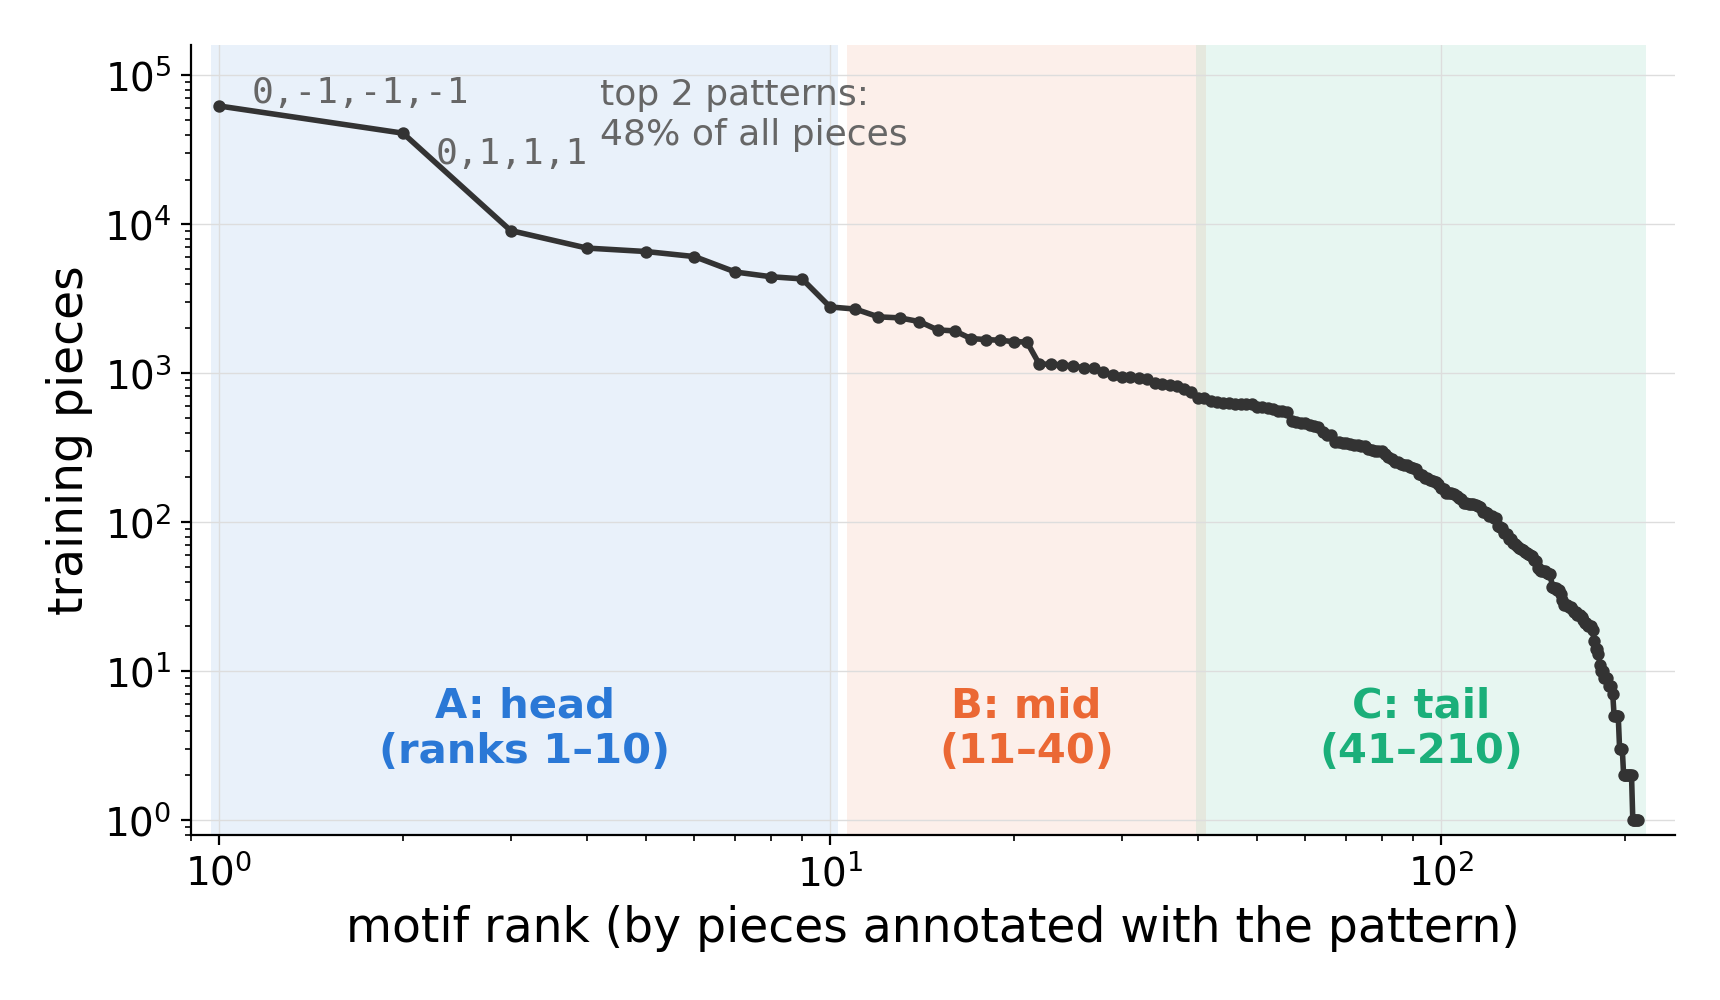
\includegraphics[width=0.85\linewidth]{fig_5_motif_zipf.png}
  \caption{Motif rank frequency over the full training corpus (log log),
  ranked by how many pieces carry each pattern as their extracted motif
  annotation. Shaded bands mark the head, mid, and tail frequency regimes
  used for evaluation sampling.}
  \label{fig:zipf}
\end{figure}

\section*{NeurIPS Paper Checklist}

%%% BEGIN INSTRUCTIONS %%%
The checklist is designed to encourage best practices for responsible machine learning research, addressing issues of reproducibility, transparency, research ethics, and societal impact. Do not remove the checklist: {\bf The papers not including the checklist will be desk rejected.} The checklist should follow the references and follow the (optional) supplemental material.  The checklist does NOT count towards the page
limit. 

Please read the checklist guidelines carefully for information on how to answer these questions. For each question in the checklist:
\begin{itemize}
    \item You should answer \answerYes{}, \answerNo{}, or \answerNA{}.
    \item \answerNA{} means either that the question is Not Applicable for that particular paper or the relevant information is Not Available.
    \item Please provide a short (1--2 sentence) justification right after your answer (even for \answerNA). 
   % \item {\bf The papers not including the checklist will be desk rejected.}
\end{itemize}

{\bf The checklist answers are an integral part of your paper submission.} They are visible to the reviewers, area chairs, senior area chairs, and ethics reviewers. You will also be asked to include it (after eventual revisions) with the final version of your paper, and its final version will be published with the paper.

The reviewers of your paper will be asked to use the checklist as one of the factors in their evaluation. While \answerYes{} is generally preferable to \answerNo{}, it is perfectly acceptable to answer \answerNo{} provided a proper justification is given (e.g., error bars are not reported because it would be too computationally expensive'' or ``we were unable to find the license for the dataset we used''). In general, answering \answerNo{} or \answerNA{} is not grounds for rejection. While the questions are phrased in a binary way, we acknowledge that the true answer is often more nuanced, so please just use your best judgment and write a justification to elaborate. All supporting evidence can appear either in the main paper or the supplemental material, provided in appendix. If you answer \answerYes{} to a question, in the justification please point to the section(s) where related material for the question can be found.

IMPORTANT, please:
\begin{itemize}
    \item {\bf Delete this instruction block, but keep the section heading ``NeurIPS Paper Checklist"},
    \item  {\bf Keep the checklist subsection headings, questions/answers and guidelines below.}
    \item {\bf Do not modify the questions and only use the provided macros for your answers}.
\end{itemize} 
 

%%% END INSTRUCTIONS %%%


\begin{enumerate}

\item {\bf Claims}
    \item[] Question: Do the main claims made in the abstract and introduction accurately reflect the paper's contributions and scope?
    \item[] Answer: \answerYes{}
    \item[] Justification: The claimed contributions (motif prompt lines with a matched train/inference attention bias, the focused-crop curriculum, and the transposition-invariant evaluator) are described in Section~\ref{sec:method}, and the headline result quoted in the abstract (92.3\% containment) is the full-model figure of Table~\ref{tab:ablation}. The stated scope (single-voice, melody-level conditioning) matches what is evaluated.
    \item[] Guidelines:
    \begin{itemize}
        \item The answer \answerNA{} means that the abstract and introduction do not include the claims made in the paper.
        \item The abstract and/or introduction should clearly state the claims made, including the contributions made in the paper and important assumptions and limitations. A \answerNo{} or \answerNA{} answer to this question will not be perceived well by the reviewers. 
        \item The claims made should match theoretical and experimental results, and reflect how much the results can be expected to generalize to other settings. 
        \item It is fine to include aspirational goals as motivation as long as it is clear that these goals are not attained by the paper. 
    \end{itemize}

\item {\bf Limitations}
    \item[] Question: Does the paper discuss the limitations of the work performed by the authors?
    \item[] Answer: \answerYes{}
    \item[] Justification: Limitations are discussed where they arise rather than in a separate section: the single-voice/monophonic scope of the model and data in Section~\ref{sec:data}, containment being a necessary but not sufficient proxy for musical use (with human evaluation deferred to future work) in Section~\ref{sec:experiments}, and the dependence of rare-motif control on the data budget in Appendix~\ref{app:scaling}.
    \item[] Guidelines:
    \begin{itemize}
        \item The answer \answerNA{} means that the paper has no limitation while the answer \answerNo{} means that the paper has limitations, but those are not discussed in the paper. 
        \item The authors are encouraged to create a separate ``Limitations'' section in their paper.
        \item The paper should point out any strong assumptions and how robust the results are to violations of these assumptions (e.g., independence assumptions, noiseless settings, model well-specification, asymptotic approximations only holding locally). The authors should reflect on how these assumptions might be violated in practice and what the implications would be.
        \item The authors should reflect on the scope of the claims made, e.g., if the approach was only tested on a few datasets or with a few runs. In general, empirical results often depend on implicit assumptions, which should be articulated.
        \item The authors should reflect on the factors that influence the performance of the approach. For example, a facial recognition algorithm may perform poorly when image resolution is low or images are taken in low lighting. Or a speech-to-text system might not be used reliably to provide closed captions for online lectures because it fails to handle technical jargon.
        \item The authors should discuss the computational efficiency of the proposed algorithms and how they scale with dataset size.
        \item If applicable, the authors should discuss possible limitations of their approach to address problems of privacy and fairness.
        \item While the authors might fear that complete honesty about limitations might be used by reviewers as grounds for rejection, a worse outcome might be that reviewers discover limitations that aren't acknowledged in the paper. The authors should use their best judgment and recognize that individual actions in favor of transparency play an important role in developing norms that preserve the integrity of the community. Reviewers will be specifically instructed to not penalize honesty concerning limitations.
    \end{itemize}

\item {\bf Theory assumptions and proofs}
    \item[] Question: For each theoretical result, does the paper provide the full set of assumptions and a complete (and correct) proof?
    \item[] Answer: \answerYes{}
    \item[] Justification: The paper's only formal claim is the transposition invariance of the motif representation; Appendix~\ref{app:extraction} defines the representation precisely (Equation~\ref{eq:classify}, Algorithm~\ref{alg:extract}), gives the argument (transposition adds a constant to every note's coordinates, leaving all pairwise differences unchanged), and corroborates it empirically with a 15-key sweep over 2{,}353 pieces.
    \item[] Guidelines:
    \begin{itemize}
        \item The answer \answerNA{} means that the paper does not include theoretical results. 
        \item All the theorems, formulas, and proofs in the paper should be numbered and cross-referenced.
        \item All assumptions should be clearly stated or referenced in the statement of any theorems.
        \item The proofs can either appear in the main paper or the supplemental material, but if they appear in the supplemental material, the authors are encouraged to provide a short proof sketch to provide intuition. 
        \item Inversely, any informal proof provided in the core of the paper should be complemented by formal proofs provided in appendix or supplemental material.
        \item Theorems and Lemmas that the proof relies upon should be properly referenced. 
    \end{itemize}

    \item {\bf Experimental result reproducibility}
    \item[] Question: Does the paper fully disclose all the information needed to reproduce the main experimental results of the paper to the extent that it affects the main claims and/or conclusions of the paper (regardless of whether the code and data are provided or not)?
    \item[] Answer: \answerYes{}
    \item[] Justification: The recipe is fully specified: prompt format and bias mechanism (Section~\ref{sec:conditioning}), curriculum and data construction (Sections~\ref{sec:curriculum}--\ref{sec:data}), training configuration and hardware (Appendix~\ref{app:curriculum_implementation}), decoding settings and evaluation protocol (Section~\ref{sec:experiments}), and the exact evaluator (Appendix~\ref{app:extraction}, released as code). The backbone checkpoint and both corpora are public.
    \item[] Guidelines:
    \begin{itemize}
        \item The answer \answerNA{} means that the paper does not include experiments.
        \item If the paper includes experiments, a \answerNo{} answer to this question will not be perceived well by the reviewers: Making the paper reproducible is important, regardless of whether the code and data are provided or not.
        \item If the contribution is a dataset and\slash or model, the authors should describe the steps taken to make their results reproducible or verifiable. 
        \item Depending on the contribution, reproducibility can be accomplished in various ways. For example, if the contribution is a novel architecture, describing the architecture fully might suffice, or if the contribution is a specific model and empirical evaluation, it may be necessary to either make it possible for others to replicate the model with the same dataset, or provide access to the model. In general. releasing code and data is often one good way to accomplish this, but reproducibility can also be provided via detailed instructions for how to replicate the results, access to a hosted model (e.g., in the case of a large language model), releasing of a model checkpoint, or other means that are appropriate to the research performed.
        \item While NeurIPS does not require releasing code, the conference does require all submissions to provide some reasonable avenue for reproducibility, which may depend on the nature of the contribution. For example
        \begin{enumerate}
            \item If the contribution is primarily a new algorithm, the paper should make it clear how to reproduce that algorithm.
            \item If the contribution is primarily a new model architecture, the paper should describe the architecture clearly and fully.
            \item If the contribution is a new model (e.g., a large language model), then there should either be a way to access this model for reproducing the results or a way to reproduce the model (e.g., with an open-source dataset or instructions for how to construct the dataset).
            \item We recognize that reproducibility may be tricky in some cases, in which case authors are welcome to describe the particular way they provide for reproducibility. In the case of closed-source models, it may be that access to the model is limited in some way (e.g., to registered users), but it should be possible for other researchers to have some path to reproducing or verifying the results.
        \end{enumerate}
    \end{itemize}


\item {\bf Open access to data and code}
    \item[] Question: Does the paper provide open access to the data and code, with sufficient instructions to faithfully reproduce the main experimental results, as described in supplemental material?
    \item[] Answer: \answerYes{}
    \item[] Justification: The evaluation code, annotated training samples, and all showcased generated pieces are released with a runnable notebook (Appendix~\ref{app:curriculum_implementation}), so the reported containment metrics can be verified directly; the training corpora are public (OpenScore Lieder, Irishman). The fine-tuned weights and training pipeline are not released with this non-archival submission, so reproducing training requires following the recipe in the paper rather than running released scripts.
    \item[] Guidelines:
    \begin{itemize}
        \item The answer \answerNA{} means that paper does not include experiments requiring code.
        \item Please see the NeurIPS code and data submission guidelines (\url{https://neurips.cc/public/guides/CodeSubmissionPolicy}) for more details.
        \item While we encourage the release of code and data, we understand that this might not be possible, so \answerNo{} is an acceptable answer. Papers cannot be rejected simply for not including code, unless this is central to the contribution (e.g., for a new open-source benchmark).
        \item The instructions should contain the exact command and environment needed to run to reproduce the results. See the NeurIPS code and data submission guidelines (\url{https://neurips.cc/public/guides/CodeSubmissionPolicy}) for more details.
        \item The authors should provide instructions on data access and preparation, including how to access the raw data, preprocessed data, intermediate data, and generated data, etc.
        \item The authors should provide scripts to reproduce all experimental results for the new proposed method and baselines. If only a subset of experiments are reproducible, they should state which ones are omitted from the script and why.
        \item At submission time, to preserve anonymity, the authors should release anonymized versions (if applicable).
        \item Providing as much information as possible in supplemental material (appended to the paper) is recommended, but including URLs to data and code is permitted.
    \end{itemize}


\item {\bf Experimental setting/details}
    \item[] Question: Does the paper specify all the training and test details (e.g., data splits, hyperparameters, how they were chosen, type of optimizer) necessary to understand the results?
    \item[] Answer: \answerYes{}
    \item[] Justification: Optimizer, learning rate, batch size, architecture, epochs, and early-stopping/checkpoint selection are given in Appendix~\ref{app:curriculum_implementation}; bias strength and its selection in Sections~\ref{sec:conditioning} and~\ref{sec:ablations}; decoding parameters, per-motif sample sizes, and the stratified motif sample in Section~\ref{sec:experiments}.
    \item[] Guidelines:
    \begin{itemize}
        \item The answer \answerNA{} means that the paper does not include experiments.
        \item The experimental setting should be presented in the core of the paper to a level of detail that is necessary to appreciate the results and make sense of them.
        \item The full details can be provided either with the code, in appendix, or as supplemental material.
    \end{itemize}

\item {\bf Experiment statistical significance}
    \item[] Question: Does the paper report error bars suitably and correctly defined or other appropriate information about the statistical significance of the experiments?
    \item[] Answer: \answerYes{}
    \item[] Justification: The main results in Table~\ref{tab:ablation} carry closed-form 95\% Wilson score intervals on the pooled binomial counts ($n{=}1200$: 24 motifs $\times$ 50 generations); the variability captured is sampling variability of the stochastic decoding, as the evaluator itself is deterministic.
    \item[] Guidelines:
    \begin{itemize}
        \item The answer \answerNA{} means that the paper does not include experiments.
        \item The authors should answer \answerYes{} if the results are accompanied by error bars, confidence intervals, or statistical significance tests, at least for the experiments that support the main claims of the paper.
        \item The factors of variability that the error bars are capturing should be clearly stated (for example, train/test split, initialization, random drawing of some parameter, or overall run with given experimental conditions).
        \item The method for calculating the error bars should be explained (closed form formula, call to a library function, bootstrap, etc.)
        \item The assumptions made should be given (e.g., Normally distributed errors).
        \item It should be clear whether the error bar is the standard deviation or the standard error of the mean.
        \item It is OK to report 1-sigma error bars, but one should state it. The authors should preferably report a 2-sigma error bar than state that they have a 96\% CI, if the hypothesis of Normality of errors is not verified.
        \item For asymmetric distributions, the authors should be careful not to show in tables or figures symmetric error bars that would yield results that are out of range (e.g., negative error rates).
        \item If error bars are reported in tables or plots, the authors should explain in the text how they were calculated and reference the corresponding figures or tables in the text.
    \end{itemize}

\item {\bf Experiments compute resources}
    \item[] Question: For each experiment, does the paper provide sufficient information on the computer resources (type of compute workers, memory, time of execution) needed to reproduce the experiments?
    \item[] Answer: \answerYes{}
    \item[] Justification: Appendix~\ref{app:curriculum_implementation} states the hardware (a single NVIDIA RTX A6000, 48\,GB, on an internal cluster), the per-run budget (under 48 GPU-hours), the estimated total for the reported grids (roughly one GPU-month), and notes that unreported exploratory runs required a comparable additional amount.
    \item[] Guidelines:
    \begin{itemize}
        \item The answer \answerNA{} means that the paper does not include experiments.
        \item The paper should indicate the type of compute workers CPU or GPU, internal cluster, or cloud provider, including relevant memory and storage.
        \item The paper should provide the amount of compute required for each of the individual experimental runs as well as estimate the total compute. 
        \item The paper should disclose whether the full research project required more compute than the experiments reported in the paper (e.g., preliminary or failed experiments that didn't make it into the paper). 
    \end{itemize}
    
\item {\bf Code of ethics}
    \item[] Question: Does the research conducted in the paper conform, in every respect, with the NeurIPS Code of Ethics \url{https://neurips.cc/public/EthicsGuidelines}?
    \item[] Answer: \answerYes{}
    \item[] Justification: The work uses public-domain or openly licensed symbolic music corpora and a publicly released backbone checkpoint, involves no human subjects or personal data, and we reviewed the Code of Ethics and found no points of conflict.
    \item[] Guidelines:
    \begin{itemize}
        \item The answer \answerNA{} means that the authors have not reviewed the NeurIPS Code of Ethics.
        \item If the authors answer \answerNo, they should explain the special circumstances that require a deviation from the Code of Ethics.
        \item The authors should make sure to preserve anonymity (e.g., if there is a special consideration due to laws or regulations in their jurisdiction).
    \end{itemize}


\item {\bf Broader impacts}
    \item[] Question: Does the paper discuss both potential positive societal impacts and negative societal impacts of the work performed?
    \item[] Answer: \answerYes{}
    \item[] Justification: Appendix~\ref{app:curriculum_implementation} (Broader impact) discusses both sides: the intended benefit of lowering the barrier for musically inclined people without formal training, and concerns about imitation and creative labor, which the composer-in-the-loop design (the human supplies the thematic material) is meant to mitigate.
    \item[] Guidelines:
    \begin{itemize}
        \item The answer \answerNA{} means that there is no societal impact of the work performed.
        \item If the authors answer \answerNA{} or \answerNo, they should explain why their work has no societal impact or why the paper does not address societal impact.
        \item Examples of negative societal impacts include potential malicious or unintended uses (e.g., disinformation, generating fake profiles, surveillance), fairness considerations (e.g., deployment of technologies that could make decisions that unfairly impact specific groups), privacy considerations, and security considerations.
        \item The conference expects that many papers will be foundational research and not tied to particular applications, let alone deployments. However, if there is a direct path to any negative applications, the authors should point it out. For example, it is legitimate to point out that an improvement in the quality of generative models could be used to generate Deepfakes for disinformation. On the other hand, it is not needed to point out that a generic algorithm for optimizing neural networks could enable people to train models that generate Deepfakes faster.
        \item The authors should consider possible harms that could arise when the technology is being used as intended and functioning correctly, harms that could arise when the technology is being used as intended but gives incorrect results, and harms following from (intentional or unintentional) misuse of the technology.
        \item If there are negative societal impacts, the authors could also discuss possible mitigation strategies (e.g., gated release of models, providing defenses in addition to attacks, mechanisms for monitoring misuse, mechanisms to monitor how a system learns from feedback over time, improving the efficiency and accessibility of ML).
    \end{itemize}
    
\item {\bf Safeguards}
    \item[] Question: Does the paper describe safeguards that have been put in place for responsible release of data or models that have a high risk for misuse (e.g., pre-trained language models, image generators, or scraped datasets)?
    \item[] Answer: \answerNA{}
    \item[] Justification: The released artifacts are a deterministic motif evaluator and symbolic scores (ABC text) derived from public-domain and openly licensed corpora; no model weights are released, and we see no high risk for misuse.
    \item[] Guidelines:
    \begin{itemize}
        \item The answer \answerNA{} means that the paper poses no such risks.
        \item Released models that have a high risk for misuse or dual-use should be released with necessary safeguards to allow for controlled use of the model, for example by requiring that users adhere to usage guidelines or restrictions to access the model or implementing safety filters. 
        \item Datasets that have been scraped from the Internet could pose safety risks. The authors should describe how they avoided releasing unsafe images.
        \item We recognize that providing effective safeguards is challenging, and many papers do not require this, but we encourage authors to take this into account and make a best faith effort.
    \end{itemize}

\item {\bf Licenses for existing assets}
    \item[] Question: Are the creators or original owners of assets (e.g., code, data, models), used in the paper, properly credited and are the license and terms of use explicitly mentioned and properly respected?
    \item[] Answer: \answerYes{}
    \item[] Justification: All assets are cited in Section~\ref{sec:data}: the NotaGen backbone \citep{wang2025notagen} is used from its public release, the OpenScore Lieder corpus \citep{gotham2022lieder} is CC0, and the Irishman corpus \citep{irishman2023} is used under the license stated on its dataset card; the release repository restates these licenses alongside the samples.
    \item[] Guidelines:
    \begin{itemize}
        \item The answer \answerNA{} means that the paper does not use existing assets.
        \item The authors should cite the original paper that produced the code package or dataset.
        \item The authors should state which version of the asset is used and, if possible, include a URL.
        \item The name of the license (e.g., CC-BY 4.0) should be included for each asset.
        \item For scraped data from a particular source (e.g., website), the copyright and terms of service of that source should be provided.
        \item If assets are released, the license, copyright information, and terms of use in the package should be provided. For popular datasets, \url{paperswithcode.com/datasets} has curated licenses for some datasets. Their licensing guide can help determine the license of a dataset.
        \item For existing datasets that are re-packaged, both the original license and the license of the derived asset (if it has changed) should be provided.
        \item If this information is not available online, the authors are encouraged to reach out to the asset's creators.
    \end{itemize}

\item {\bf New assets}
    \item[] Question: Are new assets introduced in the paper well documented and is the documentation provided alongside the assets?
    \item[] Answer: \answerYes{}
    \item[] Justification: The released repository (Appendix~\ref{app:curriculum_implementation}) documents the evaluator's API, the motif encoding, the provenance and licenses of every sample, and each generated piece's prompt via a manifest, with a runnable demonstration notebook; the demo site documents the generation settings for every showcased piece.
    \item[] Guidelines:
    \begin{itemize}
        \item The answer \answerNA{} means that the paper does not release new assets.
        \item Researchers should communicate the details of the dataset\slash code\slash model as part of their submissions via structured templates. This includes details about training, license, limitations, etc. 
        \item The paper should discuss whether and how consent was obtained from people whose asset is used.
        \item At submission time, remember to anonymize your assets (if applicable). You can either create an anonymized URL or include an anonymized zip file.
    \end{itemize}

\item {\bf Crowdsourcing and research with human subjects}
    \item[] Question: For crowdsourcing experiments and research with human subjects, does the paper include the full text of instructions given to participants and screenshots, if applicable, as well as details about compensation (if any)?
    \item[] Answer: \answerNA{}
    \item[] Justification: The paper involves no crowdsourcing or human-subject experiments; all evaluation is automatic, and a human listening study is explicitly deferred to future work (Section~\ref{sec:experiments}).
    \item[] Guidelines:
    \begin{itemize}
        \item The answer \answerNA{} means that the paper does not involve crowdsourcing nor research with human subjects.
        \item Including this information in the supplemental material is fine, but if the main contribution of the paper involves human subjects, then as much detail as possible should be included in the main paper. 
        \item According to the NeurIPS Code of Ethics, workers involved in data collection, curation, or other labor should be paid at least the minimum wage in the country of the data collector. 
    \end{itemize}

\item {\bf Institutional review board (IRB) approvals or equivalent for research with human subjects}
    \item[] Question: Does the paper describe potential risks incurred by study participants, whether such risks were disclosed to the subjects, and whether Institutional Review Board (IRB) approvals (or an equivalent approval/review based on the requirements of your country or institution) were obtained?
    \item[] Answer: \answerNA{}
    \item[] Justification: No research with human subjects was conducted.
    \item[] Guidelines:
    \begin{itemize}
        \item The answer \answerNA{} means that the paper does not involve crowdsourcing nor research with human subjects.
        \item Depending on the country in which research is conducted, IRB approval (or equivalent) may be required for any human subjects research. If you obtained IRB approval, you should clearly state this in the paper. 
        \item We recognize that the procedures for this may vary significantly between institutions and locations, and we expect authors to adhere to the NeurIPS Code of Ethics and the guidelines for their institution. 
        \item For initial submissions, do not include any information that would break anonymity (if applicable), such as the institution conducting the review.
    \end{itemize}

\item {\bf Declaration of LLM usage}
    \item[] Question: Does the paper describe the usage of LLMs if it is an important, original, or non-standard component of the core methods in this research? Note that if the LLM is used only for writing, editing, or formatting purposes and does \emph{not} impact the core methodology, scientific rigor, or originality of the research, declaration is not required.
    %this research?
    \item[] Answer: \answerYes{}
    \item[] Justification: The core method fine-tunes NotaGen, a symbolic-music model trained with the LLM paradigm, which is fully described (Sections~\ref{sec:method}--\ref{sec:data}); the case study additionally uses a general-purpose LLM (Fable 5) as a comparison baseline, with the exact prompt and settings given in Section~\ref{sec:case}.
    \item[] Guidelines:
    \begin{itemize}
        \item The answer \answerNA{} means that the core method development in this research does not involve LLMs as any important, original, or non-standard components.
        \item Please refer to our LLM policy in the NeurIPS handbook for what should or should not be described.
    \end{itemize}

\end{enumerate}


\end{document}
